\chapter{Appendix}

\section{\#42 Public Transport in the UK}


\subsection*{The reason I excluded transport lines and year data}
The decision to exclude transport lines and year data was based on several considerations. The main objective of this study was to analyze the structural properties of the UK transport networks, and including detailed line information and historical data would have added unnecessary complexity.

The provided datasets were limited to one week of data from 2011, as detailed by Gallotti et al. (2015) \cite{gallotti2015}, making it impossible to include multiple years. The datasets contained timetable information for every service departure, resulting in a voluminous and repetitive data set, complicating analysis. While Gallotti et al. used this data to study temporal network evolution, our focus was on network structure.

Handling the temporal data file, events.txt, was challenging due to its size. The only potential way to implement this would have been to reconstruct the lines from the events.txt file, which would have been extremely complex. One approach could have been to identify departure and arrival nodes and use the provided stop times to determine which nodes formed a line but that would have required advanced algorithms or machine learning techniques. 


Given these challenges, I decided to focus on the more feasible task of network structure analysis, leaving the detailed reconstruction of transport lines for future research. This approach allowed for a clear and manageable analysis of the network's structural properties





\subsection*{Additional Plots: Counties vs. TTWAs Visualization}
To provide a clearer understanding of how the population data were redistributed from counties to TTWAs, the following plots illustrate the geographical relationship between these regions.

\begin{figure}[H]
    \centering
    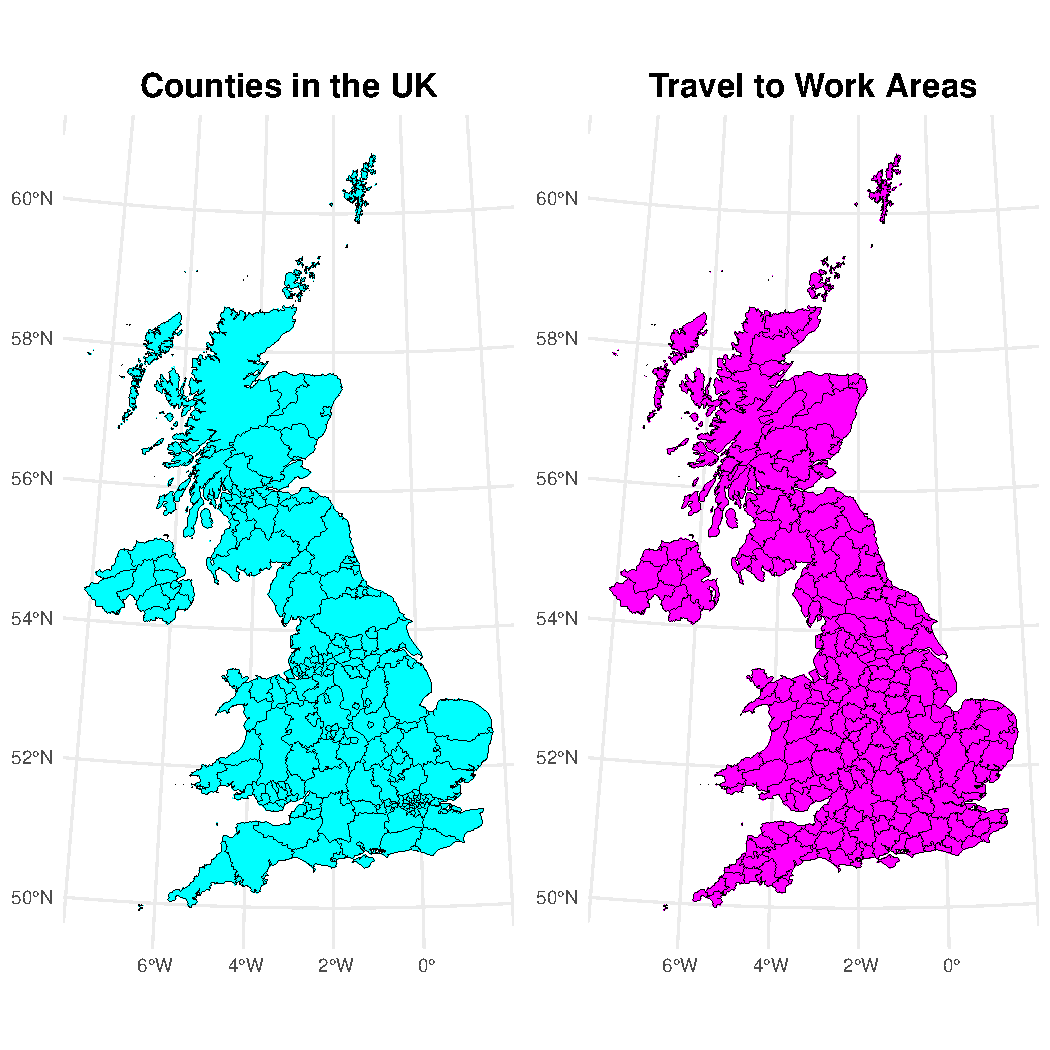
\includegraphics[width=0.55\textwidth]{images/ttwasandcounties.pdf}
    \caption{Visualization of counties and TTWAs.}
\end{figure}

\subsection*{Further Analysis of the Interlayer Network}
Further analysis of the interlayer network could provide insights into the robustness and efficiency of the UK's transport systems. This section outlines potential avenues for such analysis:

\subsubsection*{Attack Methods on Network Robustness}
Studying how different types of attacks (e.g., random failures, targeted attacks) affect the network's connectivity can reveal vulnerabilities. For example, simulating the removal of nodes or edges can help identify critical components whose failure would significantly disrupt the network.

\subsubsection*{Shortest Path Analysis Using Random Walkers}
Random walker algorithms can be employed to estimate the shortest paths within and across different transport layers. This method can highlight the efficiency of the network in terms of travel time and connectivity, providing practical insights for optimizing route planning and improving transport services.

\subsubsection*{Other Advanced Methods Studied During the Course}
Other methods such as centrality measures, community detection, and flow analysis could be applied to further dissect the network's characteristics. For instance:
\begin{itemize}
    \item \textbf{Centrality Measures:} Identifying the most influential nodes in the network based on degree centrality, betweenness centrality, or eigenvector centrality.
    \item \textbf{Community Detection:} Using algorithms like Louvain or Girvan-Newman to find clusters or communities within the network, which could correspond to functional regions or densely interconnected areas.
    \item \textbf{Flow Analysis:} Analyzing the flow of passengers or goods through the network to understand bottlenecks and optimize network performance.
\end{itemize}

These analyses can provide a deeper understanding of the transport network's dynamics and offer data-driven recommendations for enhancing its resilience and efficiency.